% ------------------------------------------------------------------------
% file `v1-exercise-2-exercise-body.tex'
%   in folder `xsim/'
%
%     exercise of type `exercise' with id `2'
%
% generated by the `exercise' environment of the
%   `xsim' package v0.21 (2022/02/12)
% from source `v1' on 2022/09/08 on line 41
% ------------------------------------------------------------------------
    Les affirmations suivantes sont-elles vraies ou fausses. Justifie dans les deux cas.
    \begin{enumerate}
        \item Le point $(4;14)$ appartient au graphe de la fonction $f(x)=3x+4$.
        \item La racine d'une fonction est le point d'intersection de la fonction avec l'axe des abscisses.
        \item $f(x) = 8$ est une fonction du premier degré.
        \item Le tableau suivant est le tableau de signe d'une fonction croissante.
        \begin{center}
            \begin{tikzpicture}
                \tkzTabInit[espcl=1.5]{$x$/0.5,$f(x)$/0.5}{$-\infty$, $r$, $+\infty$}
                \tkzTabLine{,-,z,+,}
            \end{tikzpicture}
        \end{center}
    \end{enumerate}
